\section{From ex post compensation to a credible guarantee}
\label{sec:ex-post-compensation}

A repayment guarantee can interrupt the feedback that sustains an adverse equilibrium. We first measure the losses relative to the highest-repayment outcome, then ask what financial backing makes that outcome unique. Protection is directed to interbank creditors, whose receipts enter bank clearing. Financing is external to the bank block and does not reduce banks' other resources.

\subsection{The preferred outcome and the compensation benchmark}

The preferred equilibrium $e^*(s)$ and its repayment vector $\bar{\mathbf{R}}(s)$ are defined in Section~\ref{subsec:recovery-wedge}. As the greatest fixed point, this vector dominates every other equilibrium and maximizes $\sum_jR_j^e(s)$. It can retain defaults caused by fundamental losses.

Let $L_j^{BB}=\sum_{i\in\mathcal B}x_{ij}$ be bank $j$'s debt to banking creditors, including claims among distinct institutions in the same country. If equilibrium $e$ has already occurred, compensating their shortfall relative to the preferred outcome costs
\[
 C_B(e,s)=\sum_jL_j^{BB}[\bar R_j(s)-R_j^e(s)]_+,
 \qquad [z]_+=\max\{z,0\}.
\]
For example, 40 units of debt repaid at .90 instead of .98 require compensation of $40(.98-.90)=3.2$. Extending compensation to all creditors gives $C_A(e,s)=\sum_jD_j[\bar R_j(s)-R_j^e(s)]_+$. Neither calculation changes the realized repayments.

The largest bank-creditor bill within a state is $C_{B,\max}(s)=\max_{e\in\mathcal E_0(s)}C_B(e,s)$. Its maximum across states defines
\begin{equation}
 B_{\mathrm{post}}=\max_s C_{B,\max}(s),\qquad
 b_{\mathrm{post}}=B_{\mathrm{post}}/\sum_jD_j.
 \label{eq:ex-post-compensation-bound}
\end{equation}
This maximum covers mutually exclusive states; it is not a sum or an expectation. Table~\ref{tab:ex-post-compensation} reports the bills for bank creditors and all creditors. The maximum bank-creditor bill is EUR~126 billion, or 0.61\% of aggregate clearing debt. Unique-equilibrium states have no within-state gap, although fundamental losses can remain.

\begin{table}[htbp]
\centering
\floatcaption{Maximum ex post creditor compensation within each sovereign state}{Country codes identify defaulting sovereigns; None denotes no sovereign
default. Equilibria counts banking equilibria without intervention. Banks only
reports $C_{B,\max}(s)$ and All creditors reports $\max_{e\in\mathcal E_0(s)}C_A(e,s)$,
both as percentages of aggregate bank debt, with the corresponding amounts
in EUR billions in parentheses. Percentages are rounded to two decimal
places; euro amounts are rounded to whole billions from the unrounded
compensation bills. A dash denotes zero compensation.
The largest entry in Banks only
is $b_{\mathrm{post}}$ expressed as a percentage. Transfers cover shortfalls
relative to the preferred equilibrium within the same sovereign state.}
\label{tab:ex-post-compensation}

\begin{tabular*}{\textwidth}{@{\extracolsep{\fill}}lrrr@{}}
\toprule
Sovereign defaults & Equilibria & Banks only & All creditors \\
\midrule
None & 1 & $-$ & $-$ \\
ESP & 1 & $-$ & $-$ \\
ITA & 1 & $-$ & $-$ \\
ITA+ESP & 1 & $-$ & $-$ \\
FRA & 2 & 0.35\% (\euro{}72 bn) & 2.05\% (\euro{}421 bn) \\
FRA+ESP & 2 & 0.36\% (\euro{}73 bn) & 2.11\% (\euro{}434 bn) \\
FRA+ITA & 2 & 0.36\% (\euro{}74 bn) & 2.12\% (\euro{}436 bn) \\
FRA+ITA+ESP & 2 & 0.37\% (\euro{}76 bn) & 2.19\% (\euro{}450 bn) \\
DEU & 1 & $-$ & $-$ \\
DEU+ESP & 1 & $-$ & $-$ \\
DEU+ITA & 1 & $-$ & $-$ \\
DEU+ITA+ESP & 1 & $-$ & $-$ \\
DEU+FRA & 2 & 0.35\% (\euro{}72 bn) & 2.05\% (\euro{}422 bn) \\
DEU+FRA+ESP & 2 & 0.36\% (\euro{}74 bn) & 2.11\% (\euro{}434 bn) \\
DEU+FRA+ITA & 2 & 0.36\% (\euro{}74 bn) & 2.13\% (\euro{}437 bn) \\
DEU+FRA+ITA+ESP & 3 & 0.61\% (\euro{}126 bn) & 3.71\% (\euro{}762 bn) \\
\bottomrule
\end{tabular*}

\par\smallskip

\end{table}


\subsection{A repayment floor before settlement}

After the sovereign state is observed and before banks settle, the facility promises bank creditors at least $\bar R_j(s)$ per unit lent to debtor $j$. Exposures and debts are already in place (Figure~\ref{fig:policy-timing}). If the promise is fully honoured, creditors receive $\widetilde R_j$ and the facility pays $P_j$:
\[
 \widetilde R_j=\max\{R_j,\bar R_j(s)\},\qquad
 P_j=L_j^{BB}[\bar R_j(s)-R_j]_+.
\]
Here $R_j$ is the debtor bank's own repayment under the policy.\footnote{The maximum specifies the guarantee for any candidate repayment vector: $\widetilde R_j=R_j$ when $R_j\geq\bar R_j(s)$, and the facility tops up any shortfall otherwise. Proposition~\ref{prop:greatest-floor} below proves that a fully credible floor yields $R_j=\bar R_j(s)$ in equilibrium. Hence $\widetilde R_j=R_j=\bar R_j(s)$ and transfers are zero; this equality is an equilibrium result, not an assumption in the policy rule.} Transfers go to its creditor banks and increase their receipts; nonbank creditors receive $R_j$. Replacing ordinary interbank receipts with $\widetilde R_j$ therefore changes the clearing equations. Repayments and transfers must be solved jointly.

\begin{figure}[htbp]
\centering
\floatcaption{Timing of the repayment-floor guarantee}{The recovery backstop in
Section~\ref{sec:interbank-recovery-backstop} has the same timing.}
\label{fig:policy-timing}

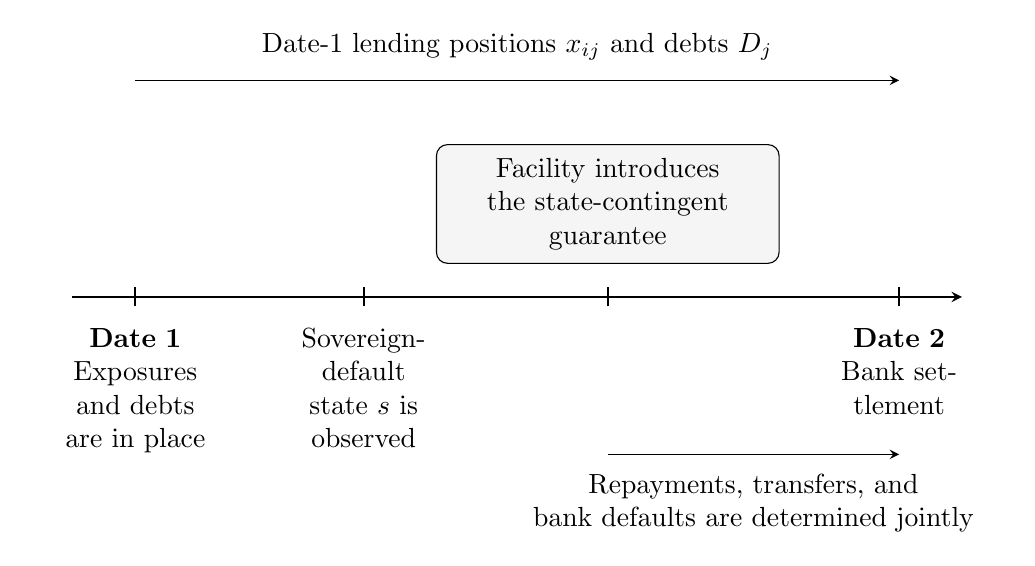
\begin{tikzpicture}[x=1cm,y=1cm,>=stealth,
  event/.style={align=center,text width=2.5cm},
  policy/.style={draw,rounded corners,align=center,text width=4.0cm,
                 inner sep=5pt,fill=black!4}]
  \draw[->,line width=0.7pt] (0,0) -- (11.3,0);
  \foreach \x in {0.8,3.7,6.8,10.5}
    \draw[line width=0.7pt] (\x,-0.12) -- (\x,0.12);

  \node[event,anchor=north] at (0.8,-0.28)
    {\textbf{Date 1}\\Exposures and debts\\are in place};
  \node[event,anchor=north] at (3.7,-0.28)
    {Sovereign-default\\state $s$ is observed};
  \node[policy,anchor=south] at (6.8,0.42)
    {Facility introduces\\the state-contingent\\guarantee};
  \node[event,anchor=north] at (10.5,-0.28)
    {\textbf{Date 2}\\Bank settlement};

  \draw[->,line width=0.5pt] (0.8,2.75) -- (10.5,2.75)
    node[midway,above=5pt,fill=white,inner sep=2pt,align=center]
    {Date-1 lending positions $x_{ij}$ and debts $D_j$};
  \draw[->,line width=0.5pt] (6.8,-2.00) -- (10.5,-2.00)
    node[midway,below=5pt,fill=white,inner sep=2pt,align=center]
    {Repayments, transfers, and\\bank defaults are determined jointly};
\end{tikzpicture}

\end{figure}

\subsection{Unique implementation and sufficient backing}
\label{sec:floor-equilibrium-effects}\label{sec:floor-sufficient-budget}

The repayment floor introduced above promises bank creditors at least the preferred-equilibrium repayment $\bar R_j(s)$ on each debtor bank. Unlike the ex post compensation calculation, this promise enters the clearing equations: protected interbank receipts increase the resources available for banks' own repayments. The question is whether this change merely reduces shortfalls or rules out the adverse equilibria altogether.

With the greatest original repayment vector $\bar{\mathbf{R}}(s)$ as target, the policy equation is $\mathbf{R}=F_s(\mathbf{R}\vee\bar{\mathbf{R}}(s))$, where $\vee$ denotes the componentwise maximum. Proposition~\ref{prop:greatest-floor} shows that, when the promise is credible, this equation has the unique solution $\mathbf{R}=\bar{\mathbf{R}}(s)$. Hence $\mathbf{R}\vee\bar{\mathbf{R}}(s)=\mathbf{R}=\bar{\mathbf{R}}(s)$: banks themselves deliver the target repayments and the facility makes no transfers. This is the coordination role of a credible guarantee \citep{DiamondDybvig1983,JacksonPernoud2021}. For now, we assume the promise is fully honoured; the financial capacity needed to support it is considered after the proposition.

\begin{proposition}[Unique equilibrium under a fully credible floor]\label{prop:greatest-floor}
Fix a sovereign state $s$, portfolios, nonbank receipts and bank repayment rules. Suppose the ordinary repayment map $F_s$ is a nondecreasing self-map of $\mathcal K=[0,1]^{|\mathcal B|}$, and let $\bar{\mathbf{R}}(s)$ be its greatest fixed point. A credible interbank repayment floor at $\bar{\mathbf{R}}(s)$, financed without reducing any bank's other resources, has the unique ordinary repayment vector $\mathbf{R}=\bar{\mathbf{R}}(s)$ and entails zero transfers in equilibrium.
\end{proposition}
\begin{proof}
At any policy equilibrium, monotonicity implies
\[
 \mathbf{R}=F_s(\mathbf{R}\vee\bar{\mathbf{R}})\geq F_s(\bar{\mathbf{R}})=\bar{\mathbf{R}}.
\]
Here and below, inequalities between repayment vectors hold componentwise. Consequently $\mathbf{R}\vee\bar{\mathbf{R}}=\mathbf{R}$, so $\mathbf{R}=F_s(\mathbf{R})$ is an original equilibrium. Since $\bar{\mathbf{R}}$ is its greatest fixed point, $\mathbf{R}\leq\bar{\mathbf{R}}$. Hence $\mathbf{R}=\bar{\mathbf{R}}$. Conversely, $\bar{\mathbf{R}}$ satisfies the policy equation with no transfer.
\end{proof}

The argument has two steps. Protected receipts ensure that every bank can repay at least as much as in the original preferred equilibrium. At such repayments no guarantee is needed, so any policy equilibrium must also be an equilibrium of the original system. Since the preferred equilibrium already has the greatest original repayments, it is the only possibility. Monotonicity is sufficient for this argument; continuity and Eisenberg--Noe regularity are not required.

In the French-only sovereign-default example, the original French bank repayments are 100\% and 94.7\%. The fully credible floor at 100\% changes banks' interbank receipts and eliminates the 94.7\% outcome: French banks themselves repay fully, with no payment by the facility. The result does not eliminate fundamental defaults. If the target includes partial repayment, as for Italian banks after Italian sovereign default alone, that partial repayment remains.

Zero equilibrium transfers do not mean that the promise requires no financial backing. Proposition~\ref{prop:greatest-floor} assumes full credibility without determining the capacity needed to sustain it. Let $B\geq0$ denote the facility's capacity. Recall that $B_{\mathrm{post}}$, defined in equation~\eqref{eq:ex-post-compensation-bound}, is the largest ex post compensation bill for bank creditors, measured relative to the preferred outcome and maximized across the original equilibria and sovereign states. The Online Appendix shows that total guarantee claims at any policy equilibrium cannot exceed $B_{\mathrm{post}}$. Capacity $B\geq B_{\mathrm{post}}$ therefore allows the facility to honour the floor in every policy equilibrium, making the preferred outcome unique by Proposition~\ref{prop:greatest-floor}. Thus the ex post compensation bill provides a sufficient commitment bound. The next subsection asks whether a smaller capacity can also make the preferred equilibrium unique, accounting for how creditors anticipate rationing.

\subsection{Minimum capacity under proportional rationing}\label{sec:minimum-floor-budget}

We fix the allocation rule: when claims exceed capacity $B$, every claimant receives the same fraction of its claim. Let $\mathbf{h}_s(\mathbf{R})=[\bar{\mathbf{R}}(s)-\mathbf{R}]_+$ be the vector of per-unit guarantee claims, with the positive part taken componentwise, and let $H_s(\mathbf{R})=\sum_jL_j^{BB}h_{s,j}(\mathbf{R})$ be their total amount. The paid fraction is $\theta_B(\mathbf{R};s)=\min\{1,B/H_s(\mathbf{R})\}$ for positive claims, and one when claims are zero. Creditors anticipate this fraction, giving
\[
 \mathbf{R}=G_{s,B}(\mathbf{R}):=F_s\bigl(\mathbf{R}+\theta_B(\mathbf{R};s)\mathbf{h}_s(\mathbf{R})\bigr).
\]
To find the critical capacity, consider equilibria at a fixed paid fraction $\theta<1$ with positive total guarantee claims:
\[
 \Gamma_s=\{(\theta,\mathbf{R}):0\leq\theta<1,\ \mathbf{R}\in\mathcal K,\ H_s(\mathbf{R})>0,\
 \mathbf{R}=F_s(\mathbf{R}+\theta \mathbf{h}_s(\mathbf{R}))\}.
\]
Each pair is an adverse outcome because the target has zero claims. Its expenditure is $\theta H_s(\mathbf{R})$; the supremum of these expenditures determines the threshold for unique implementation.

\begin{proposition}[Critical capacity for the proportional floor]\label{prop:critical-floor-budget}
Under the assumptions of Proposition~\ref{prop:greatest-floor}, define
\[
 B_s^\dagger=\sup_{(\theta,\mathbf{R})\in\Gamma_s}\theta H_s(\mathbf{R}),
 \qquad B^\dagger=\max_s B_s^\dagger,
\]
with $B_s^\dagger=0$ if $\Gamma_s$ is empty. In state $s$, every $B>B_s^\dagger$ implements $\bar{\mathbf{R}}(s)$ uniquely, whereas every $0\leq B<B_s^\dagger$ admits another equilibrium. At $B=B_s^\dagger$, uniqueness holds exactly when no pair in $\Gamma_s$ attains the supremum. The target remains an equilibrium with zero transfers at every capacity. Moreover, $B^\dagger\leq B_{\mathrm{post}}$.
\end{proposition}


The Online Appendix proves this characterization and explains how we evaluate it numerically by enumerating possible sets of defaulting banks. The guarantee rule is held fixed: the proposition does not optimize arbitrary capital injections or guaranteed links. The distinction between a critical threshold and an attained minimum matters because the distress rule can jump at equality.

In the calibration, equality implements uniquely in every state. The minimum common capacity is EUR~60.6 billion, or 0.29\% of aggregate clearing debt, 52\% below the sufficient compensation bound. The binding state has all four sovereigns defaulting. Table~\ref{tab:minimum-floor-budget} reports the state thresholds. At these capacities, every surviving outcome equals the original preferred equilibrium and transfers are zero.

\begin{table}[htbp]
\centering
\floatcaption{Minimum capacity of the proportional repayment floor and sufficient compensation bound (EUR billions)}{The matrix, OCR headroom, full accounting equity and $\lambda=.90$ are held fixed. Minimum capacities are evaluated from every admissible default regime; equality at the threshold implements uniquely under the maintained full-repayment convention. Amounts are rounded to one decimal place; comparisons and endpoint tests use unrounded values. All implementing capacities yield zero equilibrium transfers.}
\label{tab:minimum-floor-budget}

\begin{tabular*}{\textwidth}{@{\extracolsep{\fill}}lrr@{}}
\toprule
Sovereign defaults & Minimum capacity & Sufficient bound \\
\midrule
FRA & 31.7 & 71.7 \\
FRA+ESP & 42.9 & 73.5 \\
FRA+ITA & 46.6 & 74.0 \\
FRA+ITA+ESP & 59.8 & 76.2 \\
DEU+FRA & 32.2 & 71.7 \\
DEU+FRA+ESP & 43.4 & 73.6 \\
DEU+FRA+ITA & 47.4 & 74.1 \\
DEU+FRA+ITA+ESP & 60.6 & 126.3 \\
\midrule
Other eight states & 0 & 0 \\
\bottomrule
\end{tabular*}


\end{table}


These are commitment requirements, not estimates of welfare or fiscal cost. Their zero equilibrium disbursements also differ from injections that are paid and later recovered. A guarantee anticipated before exposures were formed could change saving, borrowing and investment; the fixed-exposure result and calibrated capacities do not cover those responses. We next consider a backstop whose protection depends on observed recovery losses, without a preferred-equilibrium target.
